\documentclass[12pt,a4paper]{article}
\usepackage{times}
\usepackage{mathptmx}
\usepackage{setspace}
\usepackage[utf8]{inputenc}
\usepackage[french]{babel}
\usepackage[T1]{fontenc}
\usepackage{amsmath}
\usepackage{amsfonts}
\usepackage{amssymb}
\usepackage{makeidx}
\usepackage{graphicx}
\usepackage{lmodern}
\usepackage{index}
\usepackage{diagbox}
\usepackage{multirow}
\newcommand{\HRule}{\rule{\linewidth}{0.5mm}}
\usepackage{fourier}
\usepackage[left=2cm,right=2.5cm,top=2.5cm,bottom=2.5cm]{geometry}
\author{Sarah Kaddah}
\title{Rapport de stage}
%%%%%%%%%%Interligne%%%%%%%%%%
\renewcommand{\baselinestretch}{1.5}
\begin{document}
%%%%%%%%%%%%%%%%%%%%%%%%%%%%%%%%%%%%%%%%%%%%%%%%%%%%%%%%%%%%%%%%%
%%%%%%%%%%%%%%%%%%%%%%1ere page%%%%%%%%%%%%%%%%%%%%%%%%%%%%%%%%%%
%%%%%%%%%%%%%%%%%%%%%%%%%%%%%%%%%%%%%%%%%%%%%%%%%%%%%%%%%%%%%%%%%
%%%%%%%%%%%%%%%%%%%%%%%%%%%%%%%%%%%%%%%%%%%%%%%%%%%%%%%%%%%%%%%%%
%%%%%%%%% Header %%%%%%%%%
	\begin{titlepage}
	\begin{sffamily}
	\begin{center}
	\large{Université Paris Diderot - Paris 7 \hfill 2017-2018} \bigskip
	\center{\LARGE{Master 2 Biologie-Informatique/ Bioinformatique}}	
	\begin{tabular}{c}
		\\ \\ \\
		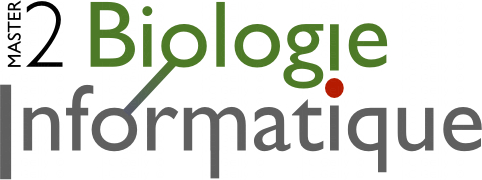
\includegraphics[scale=0.3]{img/m2.png}
	\end{tabular}
	\hfill
	\begin{tabular}{c}
		\\
		
\includegraphics[scale=0.1]{img/p7.png}
	\end{tabular}
%%%%%%%%% Title %%%%%%%%%
    \HRule \\[0.2cm]
    { \huge \bfseries \center{Etude de la fonction et des mécanismes d'évolution des séquences répétées centromériques chez les Primates}\\[0.4cm] }
    \HRule \\%[2cm]
%%%%%%%% Center %%%%%%%%
\begin{center}\LARGE{\textbf{Sarah Kaddah}}\end{center}
%%%%%%%%% Footer %%%%%%%%%
\begin{center}\Large{Tuteur: Lo\"{i}c Ponger}\end{center}~\\
\center{\large{Structure et Instabilité des Génomes}}
\center{\large{ MNHN - CNRS UMR 7196 / INSERM U1154 - Sorbonne Universités}}\\
Muséum national d'Histoire naturelle, 43 rue Cuvier 75005 PARIS \\ [1cm]
%%%%%%%%% Logos %%%%%%%%%
\begin{tabular}{cc}
	\hspace*{2.5cm} &  
	
\includegraphics[scale=0.2]{img/mnhn.jpg}
\end{tabular}
	\hfill
\begin{tabular}{c}
	
\includegraphics[scale=0.08]{img/inserm.jpg}
\end{tabular}
	\hfill
\begin{tabular}{cc}
	
\includegraphics[scale=0.08]{img/cnrs.png} &
	\hspace*{2.5cm}
\end{tabular}
	\end{center}
	\end{sffamily}
\end{titlepage}

%%%%%%%%%%%%%%%%%%%%%%%%%%%%%%%%%%%%%%%%%%%%%%%%%%%%%%%%%%%%%%%%%%
%%%%%%%%%%%%%%%%%%%%%Remerciements%%%%%%%%%%%%%%%%%%%%%%%%%%%%%%%%
%%%%%%%%%%%%%%%%%%%%%%%%%%%%%%%%%%%%%%%%%%%%%%%%%%%%%%%%%%%%%%%%%%
\section*{\begin{center}Remerciements\end{center}}~\\[0.2cm]
\addcontentsline{toc}{section}{Remerciements}
Je tiens tout d’abord à remercier énormément Loïc Ponger, responsable de mon stage, pour
son encadrement, ses conseils, ses relectures et son aide.\\

Je tiens également à remercier Christophe Escudé pour tous ses conseils et pour la
relecture mon rapport.\\

Je souhaite aussi remercier Evelyne Duvernois, pour ses conseils tant au niveau professionnel
que personnel, pour les discussions et pour les bonbons.\\

Je remercie aussi chaleureusement tout le laboratoire pour son accueil cordial.\\

Je remercie le journal club pour ces petites séances d'anglais sympathiques.\\

Je souhaite également remercier ici Catherine Etchebest et Jean-Christophe Gelly, et l’en-
semble de l’équipe pédagogique, pour cette année de master 2.\\

\thispagestyle{empty}

%%%%%%%%%%%%%%%%%%%%%%%%%%%%%%%%%%%%%%%%%%%%%%%%%%%%%%%%%%%%%%%%%%
%%%%%%%%%%%%%%%%%%%Table des matières%%%%%%%%%%%%%%%%%%%%%%%%%%%%
%%%%%%%%%%%%%%%%%%%%%%%%%%%%%%%%%%%%%%%%%%%%%%%%%%%%%%%%%%%%%%%%%
\newpage
\tableofcontents
\setcounter{page}{0}
\thispagestyle{empty}
\newpage 

%%%%%%%%%%%%%%%%%%%%%%%%%%%%%%%%%%%%%%%%%%%%%%%%%%%%%%%%%%%%%%%%
%%%%%%%%%%%%%%%%%%%%Introduction%%%%%%%%%%%%%%%%%%%%%%%%%%%%%%%%
%%%%%%%%%%%%%%%%%%%%%%%%%%%%%%%%%%%%%%%%%%%%%%%%%%%%%%%%%%%%%%%% 
\section{Introduction}
\subsection{Le centromère}
Le centromère est une structure chromatinienne qui intervient pendant la division cellulaire chez les eucaryotes. Il permet l'attachement du fuseau mitotique et la ségrégation des chromosomes \cite{Cleveland2003}.  Le kinétochore, un assemblage de protéines, trouve son cite d'attachement au niveau du centromère, auquel vont s'attacher les  microtubules aux chromosomes \cite{Santaguida2009}. La chromatine centromérique est caractérisée par la présence de la protéine CENP-A, un variant de l'histone H3, très conservé au cours de l'évolution. Celle-ci fixe la position du kinetochore par un mécanisme encore mal connu \cite{Sullivan1994}.

Bien que la fonction du centromère et des protéines sous-jacentes soient relativement bien conservées, les séquences et l'organisation du génome varie d'un taxon à l'autre. Cependant une structure commune se distingue étant de l'ADN répété en tandem, appelée ADN satellite \cite{Henikoff2001}. Ces séquences peuvent représenter environ 5\% du génome et la taille des unités de répétitions peut varier entre 7pb et 3,2kb \cite{Cellamare2009}.

\subsection{L'ADN $\alpha$-satellites}
L'ADN satellite chez les Primates est connu sous le nom d'$\alpha$-satellite. Ces séquences centromériques répétées en tandem sont riches en AT et un monomère fait 171 pb de long environ \cite{Willard1991}. Ces séquences ont été mises en évidence pour la première fois chez \textit{Chlorocebus aethiops} dans les années 1970 \cite{Kurnit1974}. des homologues ont été retrouvés chez d’autres espèces de primate \cite{Lee1997}. Néanmoins ces séquences ont été essentiellement étudiées chez l’homme.

Les séquences ont un taux d’identité qui variede  60 à 100\% \cite{Alexandrov2001}. Les séquences les plus similaires peuvent être regroupées en familles (Figure \ref{shepelev}). Ces familles résultent d'un même évènement d'amplification. Des études chez l'homme ont montré que les séquences d'une même famille se regroupaient phylogénétiquement mais aussi spatialement le long d'un chromosome \cite{Shepelev2009}. Ces observations ont permis de proposer un modèle évolutif avec des centromères en expansion. Les familles les plus récentes s’inséreraient au cœur du centromère, dans la partie active, repoussant les familles les plus anciennes jusqu'aux régions voisines, appelées péri-centromères. Les familles les plus anciennes ont une organisation monomérique tandis que les familles récentes sont sous forme d'organisation d'ordre supérieur ou \textit{Higher Order Repeat} (HOR), où un groupe de monomères appartenant à des familles différentes sont répétées en bloc les un derrière les autres ( Figure \ref{organisation_spatiale}).

\begin{figure}
	\center
		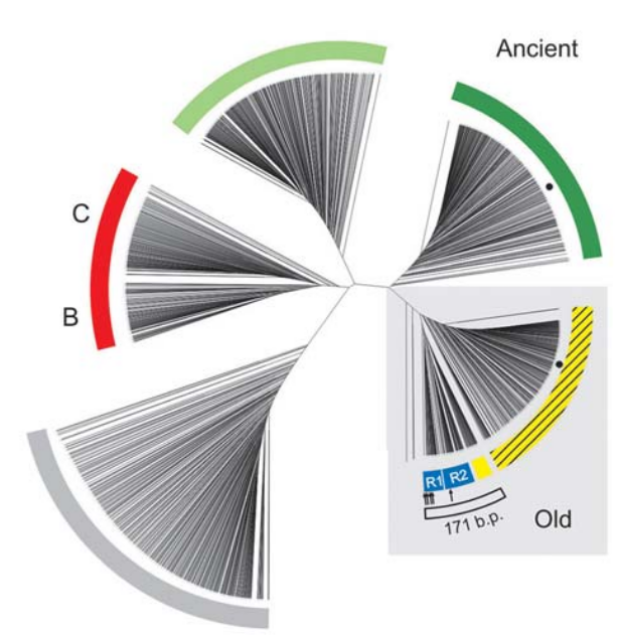
\includegraphics[height=6cm, width=6cm]{img/shepelev.png}
		\caption{\textbf{Arbre phylogénétique des séquences $\alpha$-satellites du bras p du chromosome X:} L’arbre réunit 1431 monomères présents sur le contig nt011630 \cite{Shepelev2009}.\label{shepelev}}
\end{figure}

Le rôle des $\alpha$-satellites est encore mal connu dans la fonction du centromère. Seule la protéine CENP-B serait capable de reconnaître spécifiquement un motif d'environ 17 pb (CENP-B box). Bien que cette protéine soit présente chez tous les organimes, parfois la CENP-B box est remplacée par un autre motif dans certaines familles, liant une protéine très mal caractérisée nommée pJ$\alpha$ (pJ$\alpha$ box)\cite{Romanova1996}.

\begin{figure}
	\center
		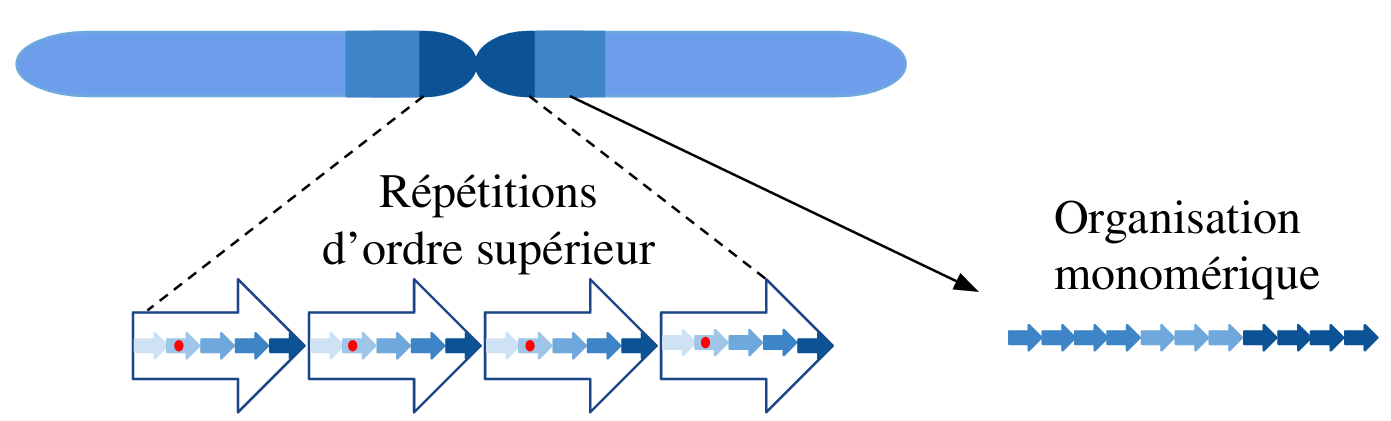
\includegraphics[height=3.5cm, width=12cm]{img/AS_organization.png}
		\caption{\textbf{Organisation spatiale des $\alpha$-satellites:} Le cœur du centromère (bleu foncé) est organisé en répétition d'ordre supérieur. Le péri-centromère (bleu clair) a une organisation monomérique. Un monomère d'une même famille est représenté par une petite flèche de même couleur. Les points rouges représentent les sites de fixation à CENP-B ou pJ$\alpha$. \label{organisation_spatiale}}
\end{figure}

\subsection{Le sujet de stage}

L'objectif de ce stage est d'étudier les $\alpha$-satellites à partir de données de séquençage haut débit afin de comprendre la fonction de ces séquences. 

Peu d'informations sur les $\alpha$-satellites existent chez les autres espèces de primates, et aucune relation inter-espèce n'a été réalisée, le séquençage et l'assemblage du génome étant difficiles. Jusqu'à présent, les études se basant sur un séquençage haut-débit ont été appliquées chez l'homme (cité ci-dessus) et chez le Gorille. L'équipe d'accueil de mon stage "ADN répété, Chromatine, Evolution" ou ARChE, a récemment développé une approche de séquençage haut débit, ciblée sur les séquences $\alpha$-satellites chez le \textit{Cercopithecus solatus} et le \textit{Cercopithecus pogonias}. Ces deux espèces ont beaucoup d'ADN satellite et de réarrangements chromosomiques et de nombreux, avec l'apparition de nombreux centromères. Cette étude a également montré les limites des approches classiques (alignements et phylogénie). Ces méthodes ne permettent pas de traiter des jeux de données conséquents, or un monomère peut avoir des milliers de copies dans un seul génome. De plus, ces méthodes non-objectives ne permettent pas de faire des comparaisons entre espèces.

Pour remédier à ce problème, une méthode de classification automatisée des $\alpha$-satellites a été implémentée en R en 2016, puis améliorée en 2017 en Python dans le laboratoire. Ce programme permet de traiter des centaines de milliers de séquences, quelque soit le nombre ou la taille des familles. De plus, cette méthode est objective et peut être appliquée à plusieurs espèces, permettant ainsi une comparaison inter-espèce des familles $\alpha$-satellites. 

Mon sujet consiste à appliquer cette méthode aux jeux de données déjà publiés pour évaluer la méthode. Dans une deuxième temps, cette méthode est appliquée à deux autres primates dans le but de  caractériser les familles d'espèces proches de primates. Les mécanismes d'évolution pourront être déduits à partir d'une comparaison inter-espèce révélant les différences et les familles communes. 

%%%%%%%%%%%%%%%%%%%%%%%%%%%%%%%%%%%%%%%%%%%%%%%%%%%%%%%%%%%%%%%%%
%%%%%%%%%%%%%%%%%%%%%%M & M%%%%%%%%%%%%%%%%%%%%%%%%%%%%%%%%%%%%%%
%%%%%%%%%%%%%%%%%%%%%%%%%%%%%%%%%%%%%%%%%%%%%%%%%%%%%%%%%%%%%%%%% 
\section{Matériel et méthode}
\subsection{Les espèces étudiées}

	\begin{figure}
		\center
		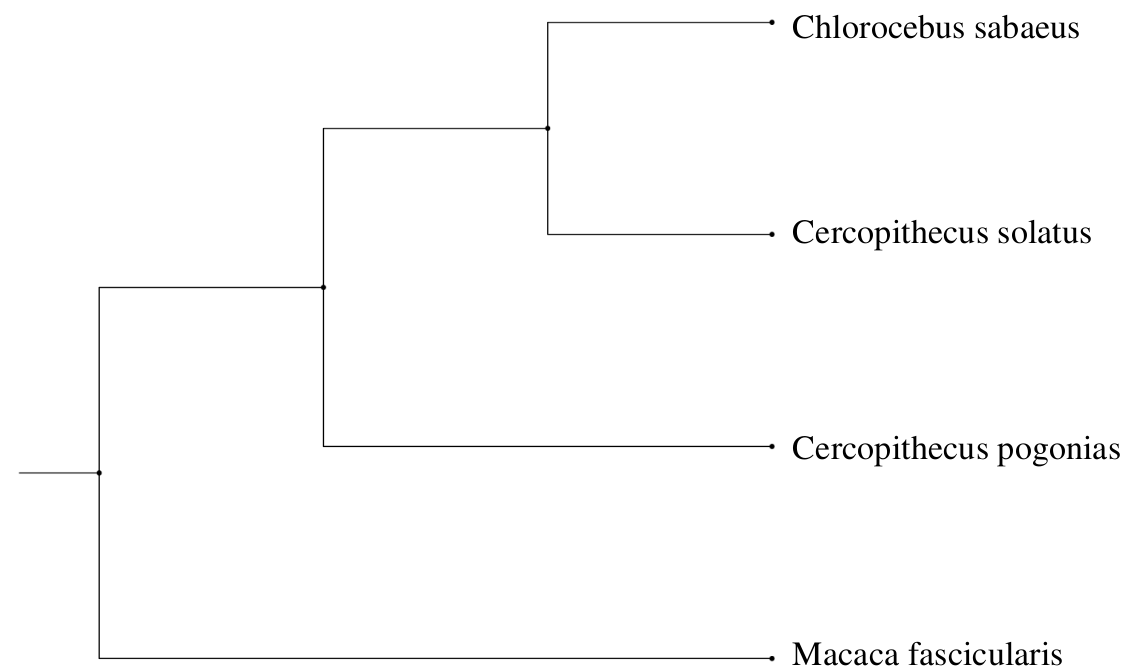
\includegraphics[height=4.5cm, width=7cm]{img/arbre_especes.png}
		\caption{\textbf{Arbre phylogénétique des espèces analysées.}\cite{Cacheux_evolution}
		\label{fig:arbre_presentation}}
	\end{figure}

Les données proviennent de reads courts environ de 171 pb, soit la taille d'un monomère. Les critères de sélection dépendent de la disponibilité des séquences de qualité parmi 10 espèces. Le \textit{C. solatus} et le \textit{C. pogonias} sont choisis ainsi que deux espèces proches (Figure \ref{fig:arbre_presentation}), le \textit{Macaca fascicularis} et le \textit{Chlorocebus sabaeus}. Tous les $\alpha$-satellites sont alignés sur les monomères de \textit{C. solatus} et \textit{C. pogonias} étudiés précédemment.

\subsection{Méthode de classification}
	\subsubsection{Principe}
Cette méthode a été développée par Florence Jornod (stage M2, 2016-2017). Elle répartit des séquences $\alpha$-satellites en familles selon la similarité. La classification est hiérarchique dichotomique. Au départ, une table contenant les fréquences des 5-mers est calculée pour chaque monomère. Ensuite une boucle itérative est exécutée pour séparer les séquences en groupes tant que les nouveaux groupes formés sont divisibles.

	\subsubsection{Répartition itérative}
Une Analyse en Composante Principale (ACP) est effectuée sur la table des fréquences des 5-mers afin de réduire les dimensions du jeu de données et d’obtenir des variables indépendantes. Des distances euclidiennes sont calculées entre toutes les paires de séquence dans l’espace défini par les premières composantes de l’ACP. 

A partir du calcul de distance, les séquences sont séparées en deux classes en utilisant la classification hiérarchique basée sur la méthode de Ward. Cette méthode maximise l’inertie interclasse. La classification hiérarchique fait un usage important de la mémoire. Par conséquent, pour traiter des jeux de données importants de plus de 100 000 séquences, l’Analyse Discriminante Linéaire , une méthode d’apprentissage, est utilisée sur un sous jeu de données formé par de 100 000 séquences tirées aléatoirement, dans ces analyses. Le modèle construit est alors appliqué sur toutes les séquences.

	\subsubsection{Double-validation d'un sous-groupe}
Le premier critère de validation est la taille du sous-groupe. Si un groupe atteint 100 séquences, il n'est pas redivisé. Le deuxième critère de validation s'appuie sur le \textit{matepair}. Ce terme correspond à la proportion de monomères ayant son plus proche voisin dans la même classe, se basant sur les distances euclidiennes calculées auparavant. Des valeurs \textit{matepairs} élevées (proches de 1) indiquent des sous-groupes bien homogènes et séparés validant la classification tandis qu’un seuil \textit{matepair} plus faible (proche de 0) entraîne plus de classes.

Un seuil de \textit{matepair} est fixé à 0.90, pour avoir des groupes homogènes. Si au moins une des valeurs de \textit{matepair} est au-dessous de ce seuil, les sous-groupes sont considérés comme formant un seul groupe et le groupe initial est sauvegardé comme une famille unique. Si les \textit{matepairs} sont au-dessus d’un certain seuil, les deux sous-groupes sont ajoutés séparément à la file pour être potentiellement redivisés ultérieurement.

	\subsection{Analyse des séquences}
	
Les séquences monomériques sont comparées à partir de leur composition en 5-mers dans le but d'identifier des regroupements d'$\alpha$-satellites sans passer par l'étape d'alignement. Pour chaque ensemble de monomères,	la table de fréquence des 5-mers est analysé en utilisant l'Analyse en composante principale pour réduire l'espace de complexité pour pourvoir visualiser les données sur les premiers plans factoriels.
	
L'alignement des séquences est fait avec muscle \cite{Edgar2004} et visualisé avec Seaview (problème de biblio UTF8). La phylogénie est construite avec la méthode du maximum de vraisemblance (PhyML) \cite{Guindon2009}. Le modèle F84 est utilisé pour la construction de l'arbre. Le support de branche est aLRT (SH-like). La fréquence d'équilibre des nucléotides, le ratio de transition et de transversion et les taux de variation sont optimisés.

Les consensus sont obtenus avec des scripts développés par l'équipe. Les motifs CENP-B (TTCGTTGGAA[AG]CGGGA), PJ$\alpha$ (TTCCTTTT[CT]CACC[AG]TAG) et pK$\beta$ (CTATAGGGCCAAAGGAA) ont été identifiés avec le logiciel fuzznuc (package EMBOSS) \cite{Rice2000} et en autorisant 2 différences au maximum par rapport au consensus.

%%%%%%%%%%%%%%%%%%%%%%%%%%%%%%%%%%%%%%%%%%%%%%%%%%%%%%%%%%%%%%%%%
%%%%%%%%%%%%%%%%%%%%%%Résultats 1%%%%%%%%%%%%%%%%%%%%%%%%%%%%%%%%
%%%%%%%%%%%%%%%%%%%%%%%%%%%%%%%%%%%%%%%%%%%%%%%%%%%%%%%%%%%%%%%%% 
\section{Résultats}
	\subsection{Caractérisation intraspécifique des familles}
	Les séquences ont été classées en utilisant une méthode de classification objective développée dans l'équipe. Le nombre de familles est déterminé indirectement par un critère sélectionnant des classes à la fois homogène et différentes les unes des autres.
	
			\subsubsection{Identification des familles}
	
				\begin{table}
			\center
			\begin{tabular}{|c|c|c|c|c|}
   			\hline
  			\textbf{Espèce} & \textbf{Nb séq tot} & \textbf{Nb fam tot} & \textbf{Nb fam > 100 séq} & \textbf{\%  seq analysé}\\
  		    \hline
   			\textit{C. solatus} & 105 529 & 564 & 12 & 96.03  \\
   			\hline
    		\textit{C. pogonias} & 112 902 & 132 & 13 & 98.71\\
   			\hline
   			\textit{C. sabaeus} & 29 842 & 338 & 43 & 89.11\\
   			\hline
   			\textit{M. fascicularis} & 235 535 & 3694 & 114 & 88.94\\
   			\hline			
			\end{tabular}
			\caption{Résumé du jeu de données et des résultats de la classification.}
			\label{tab_res}
		\end{table}
		
		\begin{figure}
			\center
			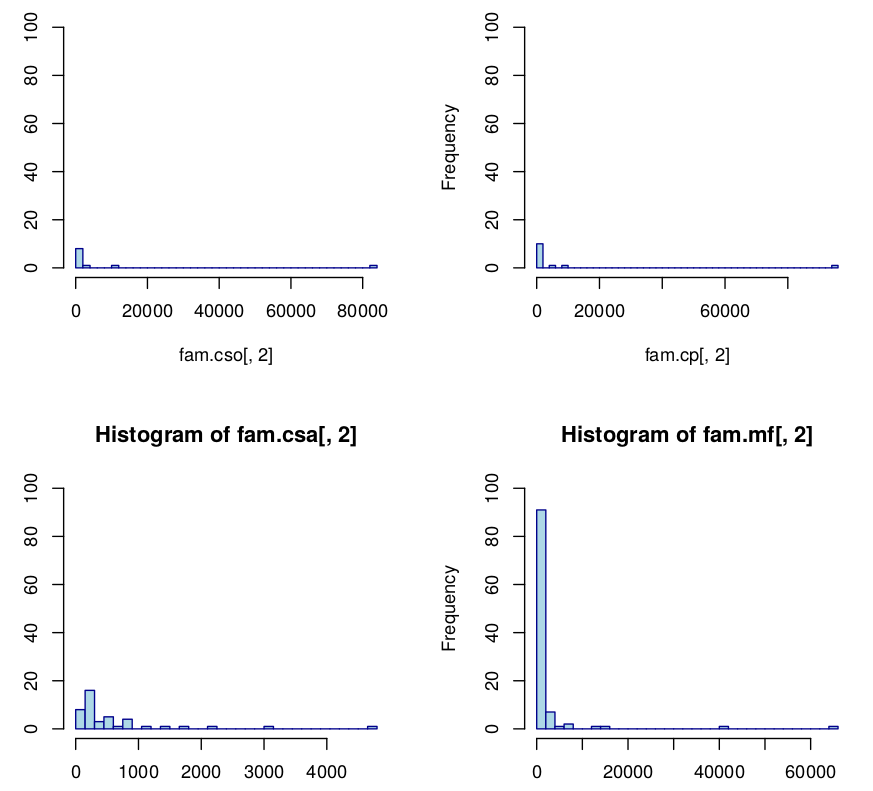
\includegraphics[scale=0.45]{img/distribution_familles.png}
			\caption{\textbf{Distribution des familles en fonction du nombre de séquences.}}
			\label{dist_fam} 
		\end{figure}

	A l'issue de la classification, seules les familles ayant plus de 100 séquences, appelées grandes familles, sont conservées pour l'analyse. Le nombre de familles conservées diminue considérablement après élimination des petites familles (<100 séquences) mais ces familles ne représentent que 11\% du jeu de données au plus (Tableau \ref{tab_res}). Malgré le nombre de familles qui diffère d'une espèce à l'autre, la distribution des familles est similaire chez les quatre espèces. Les plus petites familles sont très nombreuses et et la fréquence diminue quand la taille augmente (Figure \ref{dist_fam}). 

		\begin{figure}	
			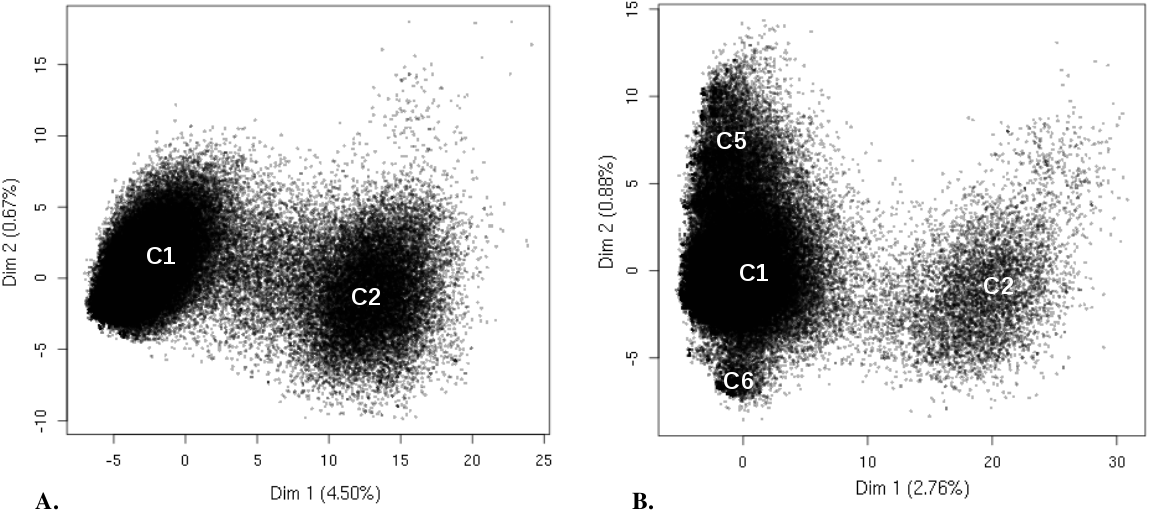
\includegraphics[scale=0.4]{img/ACP_experimental.png}  \\
			\caption{\textbf{Caractérisation visuelle des familles $\alpha$-satellite chez \textit{C. solatus} et \textit{C. pogonias} à partir d'une ACP, basée sur la composition en 5-mers des monomères :}Le nom des familles est indiqué sur les graphiques. Un point représente un monomère. \textbf{A.} \textit{C. solatus}. \textbf{B.} \textit{C. pogonias}.}
			\label{fig:ACP_exp} 
	\end{figure}	
	
	Les espèces \textit{C. solatus} et \textit{C. pogonias} sont analysées dans un premier temps pour comparer la classification automatisée avec la classification empirique (citer cacheux et al, PB UTF8). Ces familles ont été définies manuellement à partir d'une ACP basée sur la composition en 5-mers de tous les monomères (Fig. \ref{fig:ACP_exp}).Expérimentalement, 6 familles $\alpha$-satellites ont été définies empiriquement et confirmé expérimentalement chez les Cercopithèques. Ces deux espèces partagent deux grandes familles monomériques, C1 et C2, et deux familles formant un HOR d'ordre 2, C3-C4, de l'ordre d'une centaine de séquences chacune. Le \textit{C. pogonias} possède les familles supplémentaires C5 et C6.
	
		\begin{table}
			\center
			\begin{tabular}{|c|c|c|}
	    	\hline
			\textbf{Classification publiée} &  \textbf{\textit{C. solatus}}  & \textbf{\textit{C. pogonias}}\\
			\hline
			C1 &  1  & 10\\
			\hline
			C2 & 11  & 1 \\
			\hline
			C3 & 1* & 1 \\
			\hline
			C4 & 1* & 1* \\
			\hline
			C5 & - 	 &  1 \\
			\hline
			C6 & -   &  0 \\
			\hline
			\textbf{Total} & 12 + 2* < 100 seq  &  13 + 1* <100 seq \\
			\hline
		\end{tabular}
		\caption{\textbf{Comparaison des classifications automatiques avec celles publiées précedemment (Cacheux et al, 2016 et 2018)}}
		\label{tab_count_fam}
	\end{table}
		
	Bien que le nombre de grandes familles soit relativement proche entre ces deux espèces, les résultats diffèrent significativement (Tableau \ref{tab_count_fam}). Toutes les familles chez le \textit{C. solatus} sont retrouvées: 11 familles forment la famille C2, une famille forme la famille C1 et les familles C3 et C4 sont retrouvées dans des petites familles d'environ 80 séquences chacune. Chez \textit{C. pogonias}, toutes les familles sont retrouvées sauf la famille C6. La famille C1 est répartie en 10 familles, les familles C2, C3 et C5 sont retrouvées entièrement, la famille C4 est également retrouvée sous la forme d'une petite famille de 86 séquences. Chez le \textit{C. solatus}, la famille C2 est divisée en plusieurs familles et la famille C1 est retrouvée dans une seule famille. La situation inverse est retrouvée  chez \textit{C. pogonias}.
		\begin{figure}	
			\begin{tabular}{cc|cc}
				  & \textit{C. solatus} &  &  \textit{C. pogonias}\\
		\textbf{A} & 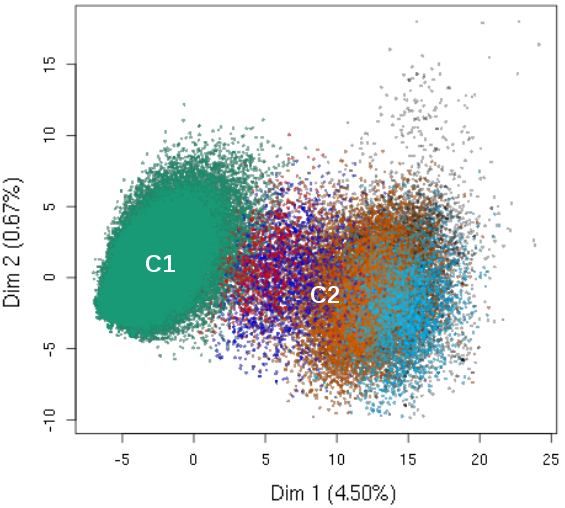
\includegraphics[scale=0.35]{img/solatus_ACP1.png} & \textbf{C} & 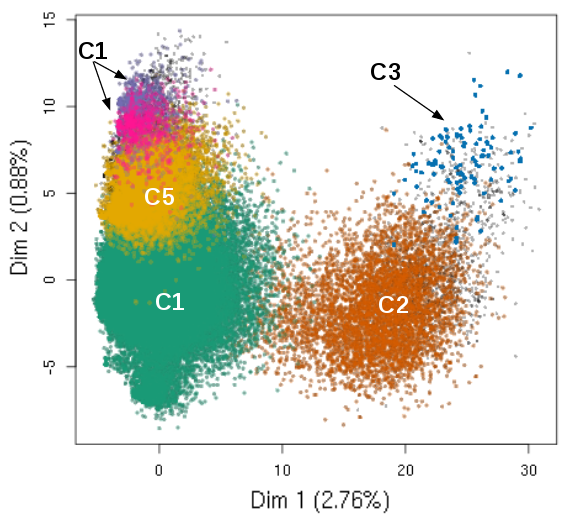
\includegraphics[scale=0.35]{img/pogonias_ACP1.png} \\
		\textbf{B} & 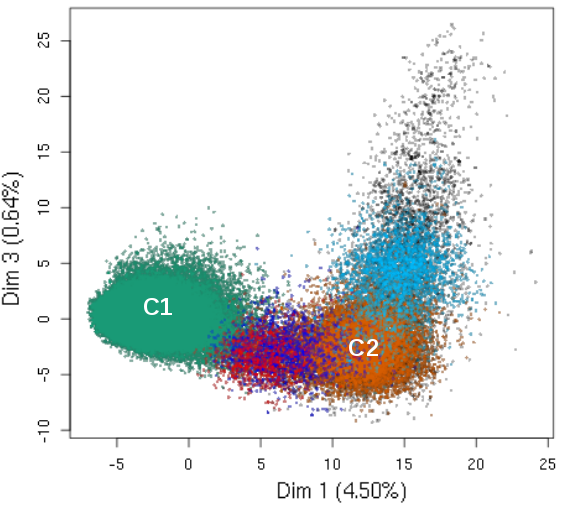
\includegraphics[scale=0.35]{img/solatus_ACP2.png} &  \textbf{D} & 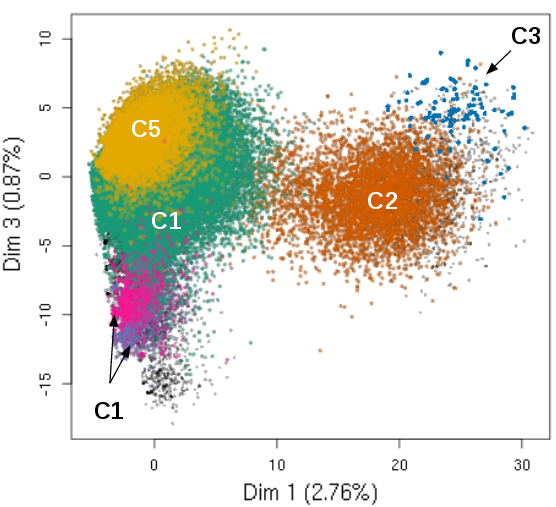
\includegraphics[scale=0.35]{img/pogonias_ACP2.png} \\
		\textbf{E} & 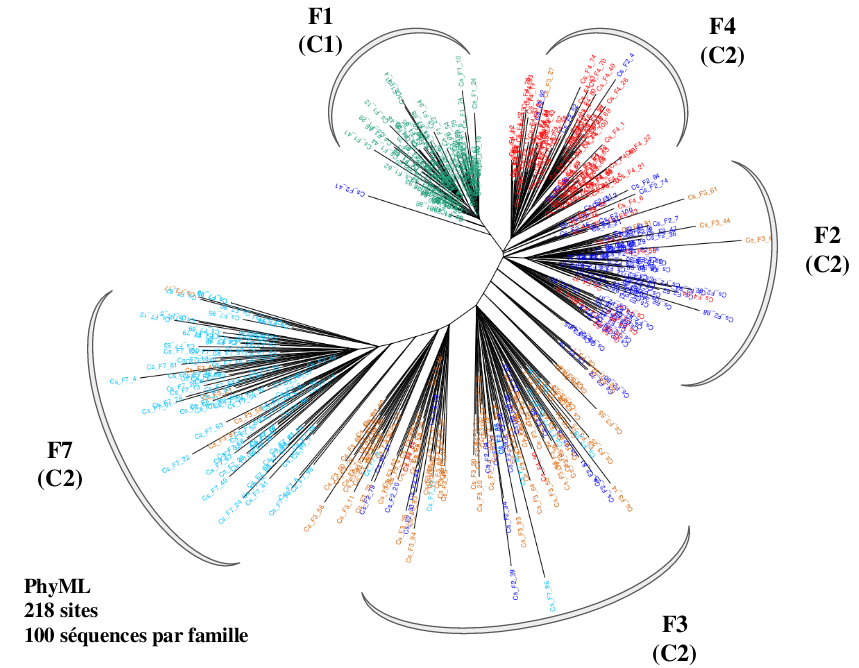
\includegraphics[scale=0.20]{img/tree_solatus.png} & \textbf{F} & 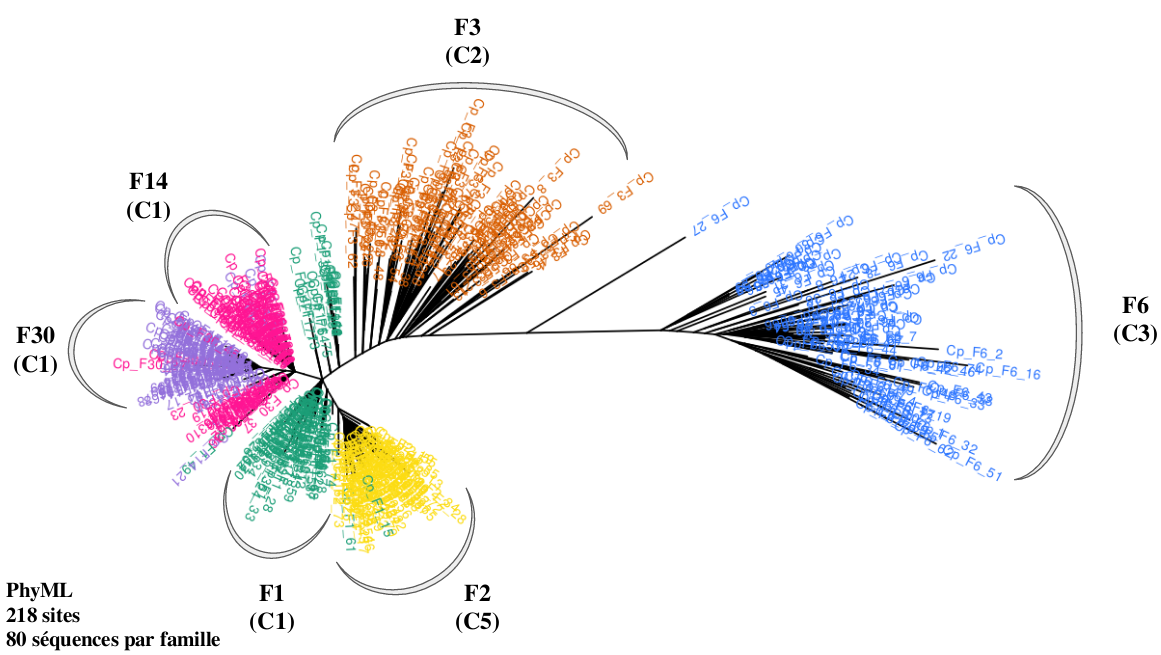
\includegraphics[scale=0.20]{img/tree_pogonias.png} \\
	\end{tabular}
	\caption{\textbf{Représentation des plus grandes familles issues de la classification automatisée:} Ces familles sont superposées sur les représentations de l'ACP des 5-mers.
	\textbf{A.} Composantes 1 et 2 de l'ACP. Les familles qui correspondraient à C1 sont en vert, C2 en orange, rouge, bleu et turquoise.  \textbf{B.} Composantes 1 et 3 de l'ACP. 
	\textbf{C.} Composantes 1 et 2 de l'ACP. Les familles qui correspondraient à C1 sont en vert, violet et rose, C2 en orange, C4 en bleu clair et C5 en jaune.
	\textbf{C.} Composantes 1 et 3 de l'ACP.
	\textbf{E. et F.} Phylogénie des différentes familles chez \textit{C. solatus} (100 séquences par famille) et \textit{C. pogonias} (80 séquences par famille) respectivement. Les couleurs sont respectivement conservées.	 
	\label{fig:so_po_acp_tree}
		} 
\end{figure}
			
			La diversité de ces familles a été analysée avec une ACP basée sur sur la composition en 5-mers (Figure \ref{fig:so_po_acp_tree}). Afin de valider la surclusterisation observée de la famille C2 chez \textit{C. solatus}. On observe toutefois une sur-clusterisation de certaines familles dont la pertinence est confirmée par l'ACP ou les phylogénies. Chez \textit{C. solatus}, la famille C1 est entièrement retrouvée dans une famille. La famille C2 est répartie en plusieurs familles. Deux familles intermédiaires (rouge et bleue) sont visibles entre la famille C1 (vert)  et C2 (orange). Elles ne sont pas distinctes.  Une famille supplémentaire (turquoise) se démarque. Pour confirmer cette division de la famille C2, la visualisation de l'ACP des 5-mers est observée en fonction des composantes 1 et 3. Les familles intermédiaires sont toujours confondues, contrairement à la famille turquoise qui forme une famille à part entière. Pour certifier ce fait, l'arbre construit atteste que chaque famille est bien retrouvée, notamment les familles intermédiaires qui forment bien deux familles. Chez \textit{C. pogonias}, les familles C2, C4 et C5 sont bien retrouvées. La famille C6 se fond dans la famille C1 (en vert). La famille C1 est divisée en deux familles supplémentaires (rose et violet). La visualisation des composantes 1 et 3 de l'ACP ne permet pas de trancher sur la classification. L'arbre montre que les familles en rose et violet sont très proches.  
			
			La classification automatique permet de retrouver les familles identifiées dans les travaux, excepté la famille C6.
			 
			\subsubsection{Motifs potentiellement fonctionnels}
\begin{figure}
	\center	
	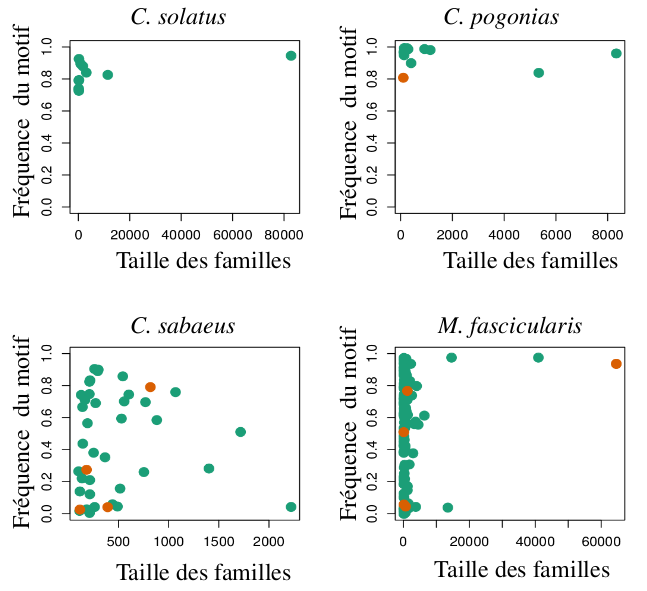
\includegraphics[scale=0.4]{img/graphique_motifs.png}
	\caption{\textbf{Fréquences des motifs CENP-B, pJ$\alpha$ ou pK$\beta$ dans les familles:} Les motifs ont été cherchés sur la base de leur consensus en autorisant deux différences. Le pourcentage de séquences par famille ayant le motif pJ$\alpha$ est en vert, pK$\beta$ en orange et CENP-B est absent de toutes les familles. Chaque famille est représentée en fonction de sa taille.
	\label{fig:motif}} 
\end{figure}
			
			La protéine CENP-B est présente chez toutes les espèces, mais les Cercopithèques ne possèdent pas son site de liaison. La protéine pJ$\alpha$ est une protéine peu connue mais dont le site de liaison est déterminé. Le motif pK$\beta$ est un site commun aux familles n'ayant ni CENP-B ni pJ$\alpha$. Ces trois motifs sont recherchés pour chaque famille de chaque espèce sur la base des consensus (partie matériel et méthodes) avec 2 mismatchs autorisés dans le but de caractériser ces familles. En effet, CENP-B est absent chez \textit{C. solatus} et \textit{C. pogonias}. Le \textit{C. sabaeus} et le \textit{M. fascicularis} n'ont pas ce motif non plus. Par contre plus de 90\% des familles chez les quatre espèces ont le motif pJ$\alpha$ mais à des niveaux différents.
			
		La totalité des familles chez \textit{C. solatus} ont le motif, dont 8 à plus de 75\%. Chez le \textit{C. pogonias}, 12 familles sur 13 ont le motif à plus de 75\%. Par ailleurs, la plus grande famille, C1, ayant plus de 80 000 séquences chez ces deux espèces, se démarque avec un pourcentage à 95\%. Le \textit{C. sabaeus} présente 39 familles avec ce motif, dont 7 l'ayant à plus de 75\%. Le \textit{M. fascicularis} a des pourcentages pour le motif pJ$\alpha$ qui varie entre 1\% et 97\%. Cette espèce a 28 familles avec le motif à plus de 75\% dont une famille de  40 000 séquences et une autre de 14 000 séquences.
		
			Le motif pK$\beta$ est présent lorsque pJ$\alpha$ est absent de la famille. Il est absent chez \textit{C. solatus}. Seule la famille C3 a ce motif à 80\% chez \textit{C. pogonias}. Le \textit{C. sabaeus} a quatre familles avec le motif, dont deux à 79\% et l'autre à 29\%. Le \textit{M. fascicularis} a cinq familles avec ce motif. La famille ayant le motif à 93\% est une grande famille de 64 000 séquences. Les deux autres familles ont le motif à 0.76\% et 0.50\%.
			
			Les quatre espèces ont des points en commun concernant l'absence du motif CENP-B et quelques familles ayant pK$\beta$. Cependant pour le motif pJ$\alpha$, les \textit{C. solatus} et \textit{C. pogonias} ont des pourcentages relativement proches mais qui diffèrent du \textit{M. fascicularis} et du \textit{C. sabaeus}, dont les valeurs sont intermédiaires. Chaque famille a un motif pour toutes les espèces excepté le \textit{M. fascicularis} qui a 6 familles sans motifs.
				
			\subsubsection{Similarité entre familles}
\begin{figure}	
	\center
	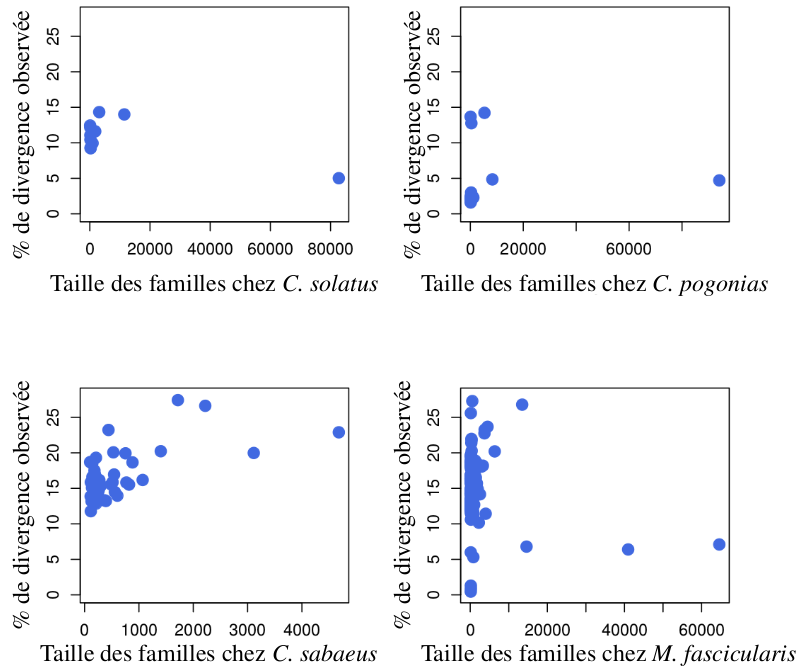
\includegraphics[scale=0.4]{img/graphique_similarity.png}
	\caption{\textbf{Pourcentage de divergence observée de chaque famille:}
	Un point correspond à une famille et son pourcentage de divergence observé.
	\label{fig:divergence}
		} 
\end{figure}
	Le pourcentage de divergence observée par famille est calculé sur 500 séquences tirées aléatoirement dans une famille. Elle permettrait d'estimer l'âge de ces familles. Les \textit{C. solatus} et \textit{C. pogonias} ont des pourcentages relativement faibles ne dépassant pas 15\%, le \textit{M. fascicularis} a des valeurs intermédiaires variant de 0.1\% à 28\%, et \textit{C. sabaeus} a les valeurs les plus élevées allant de 11\% à 28\%.
	
	Les familles qui correspondraient aux familles C1 et C5 ont un pourcentage autour de 5\%. Les autres familles chez \textit{C. solatus} ont une moyenne de 10.85\% de divergence observée. Les familles de taille moyenne (quelques centaines de séquences) qui correspondraient à la famille C1 ont des pourcentages inférieurs à 3\% chez \textit{C. pogonias} et les trois familles restantes ont des valeurs de 13\% en moyenne. Les familles du \textit{C. sabaeus} ont en moyenne 16.8\% de divergence observée, la taille n'ayant aucun rapport au pourcentage. Le \textit{M. fascicularis} a trois familles avec un pourcentage inférieur à 1\% et cinq familles à 6\% en moyenne. Les 106 familles restantes ont un pourcentage supérieur à 10\%.
	
	Le pourcentage de similarité est semblable chez les \textit{C. solatus} et \textit{C. pogonias}. Le \textit{M. fascicularis} a  quelques familles qui ont des pourcentages faibles mais il a également beaucoup de familles aux pourcentages très élevés, tandis que la majorité des familles chez le \textit{C. sabaeus} a grands pourcentages.
	
%%%%%%%%%%%%%%%%%%%%%%%%%%%%%%%%%%%%%%%%%%%%%%%%%%%%%%%%%%%%%%%%%
%%%%%%%%%%%%%%%%%%%%%%Résultats 2%%%%%%%%%%%%%%%%%%%%%%%%%%%%%%%%
%%%%%%%%%%%%%%%%%%%%%%%%%%%%%%%%%%%%%%%%%%%%%%%%%%%%%%%%%%%%%%%%% 
	\subsection{Comparaison inter-espèce}
	Pour étudier les mécanismes d'évolution des $\alpha$-satellites, une classification inter-espèce ou "super-classification" (SC) permet de comprendre les différences entre espèces. Pour chaque espèce, 100 séquences par grande famille (> 100 séquences) sont tirées aléatoirement. Un jeu de données de 18 100 séquences est soumis à la classification automatique. A l'issue de cette super-classification, 158 familles sont obtenues au total, dont 90 grandes familles. Les petites familles de moins de 20 séquences, soit 1.76\% de ce jeu de données, ne sont pas prises en compte dans l'analyse.
	
	\subsubsection{Répartition des super-familles}
	Parmi les super-familles (SF), 38 ont une taille comprise entre 100 et 20 compris, et trois familles ont une taille strictement supérieure à 800 séquences. Seule une SF \textit{a priori} est commune aux quatre espèces. Elle rassemble 6 familles parmi les 10 familles classées C2 de \textit{C. solatus} et les deux familles également classées C2 de \textit{C. pogonias}, ainsi que deux familles du \textit{M. fascicularis} et une famille du \textit{C. sabaeus}. Une partie de la famille annotée C2 serait donc commune aux quatre espèces.
	
	Une SF est partagée entre le \textit{C. pogonias}, le \textit{C. sabaeus} et le \textit{M. fascicularis}. Cette SF regroupe des familles ayant le motif pK$\beta$ et qui correspondrait à la famille C3 commune au \textit{C. pogonias} et au \textit{C. solatus}. Cela signifierait que la famille C3 serait commune à ces quatre espèces également.
	
	Certaines SF sont spécifiques aux espèces. Au sein des 8 SF spécifiques du \textit{C. pogonias}, seule l'une d'entre elles regroupe deux familles, le reste étant composé d'une famille. Elles correspondraient aux familles C5, une petite partie de C6 et essentiellement à C1. Les trois SF spécifiques de \textit{C. solatus} seraient équivalentes aux familles C2. Le \textit{C. sabaeus} en a 3 et le \textit{M. fascicularis} 27.
	
	Le \textit{C. sabaeus} et le \textit{M. fascicularis} partagent 38 SF, soit 42\% des grandes SF (> 20 séquences), dont la plus grande faisant une taille de 1194 séquences. Une seule SF est uniquement commune à \textit{C. solatus} et \textit{C. pogonias} et elle regroupe les deux plus grandes familles qui seraient du C1.
	
	\subsubsection{Une mosaïque de familles C2}
			\begin{figure}
			\center	
			\begin{tabular}{cccc}
		\textbf{A.} & 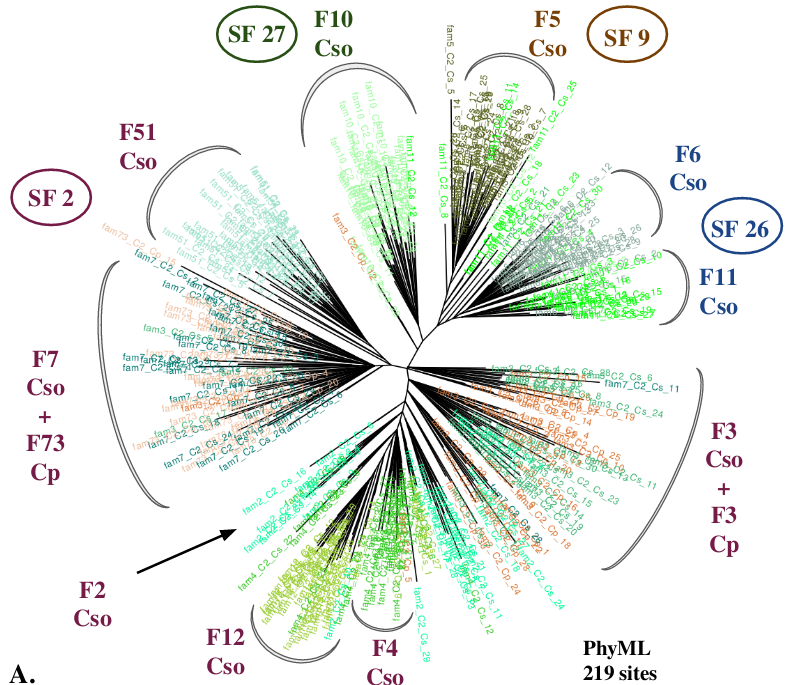
\includegraphics[scale=0.30]{img/tree_C2_pogonias_solatus.png} & \textbf{B.} & 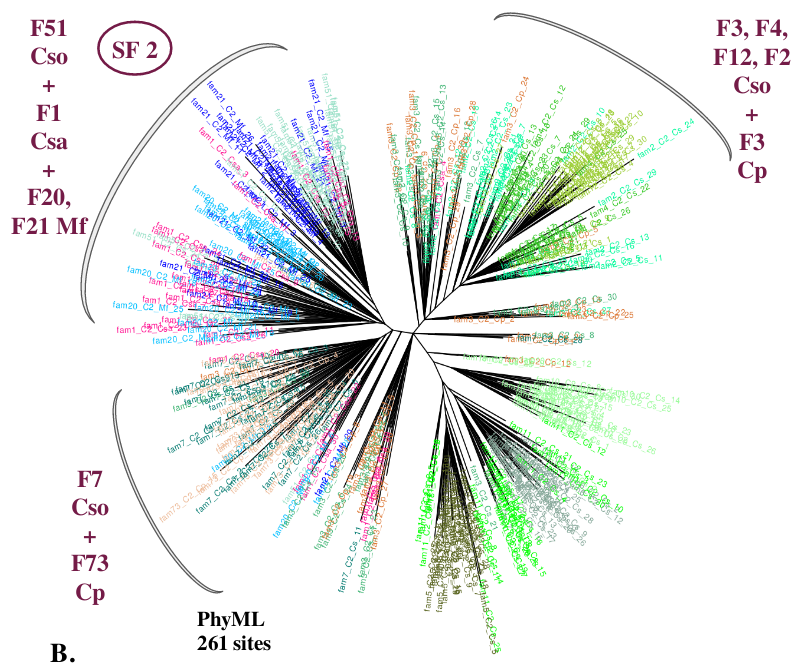
\includegraphics[scale=0.30]{img/tree_C2_all_species.png} \\
	\end{tabular}
	\caption{\textbf{Phylogénie des différentes familles qui correspondraient à la famille C2:}
	\textbf{A.}\textit{C. solatus} (tons verts) et \textit{C. pogonias} (tons orange) \textbf{B.} Des familles du \textit{M. fascicularis} (tons bleus) et \textit{C. sabeus} (rose) sont rajoutées.	 
	\label{tree_C2}} 
\end{figure}

		La famille C2 fait l'objet d'une séparation en plusieurs familles intéressantes. Pour vérifier les résultats de cette SC, 30 séquences de chacune des familles annotées C2 de \textit{C. solatus} et \textit{C. pogonias} sont tirées aléatoirement et un arbre est construit pour voir si cette division est retrouvée. Un autre arbre,  avec les familles des deux autres espèces supposées de la famille C2,  est construit.
		
		Une partie de ces familles est spécifique au \textit{C. solatus}, tandis que les familles restantes sont communes aux quatre espèces selon la classification. Dans la phylogénie, les SF 27, 9 et 26 sont bien retrouvées. Cependant la SF 2 regroupe trop de familles, sans faire de distinction (Figure \ref{tree_C2} A). Les familles présumées C2 des deux autres espèces se mélangent plus spécifiquement avec la famille 51 de \textit{C. solatus}.
						
	\subsubsection{Origine du motif pK$\beta$}
	
	\begin{figure}	
			\centering
				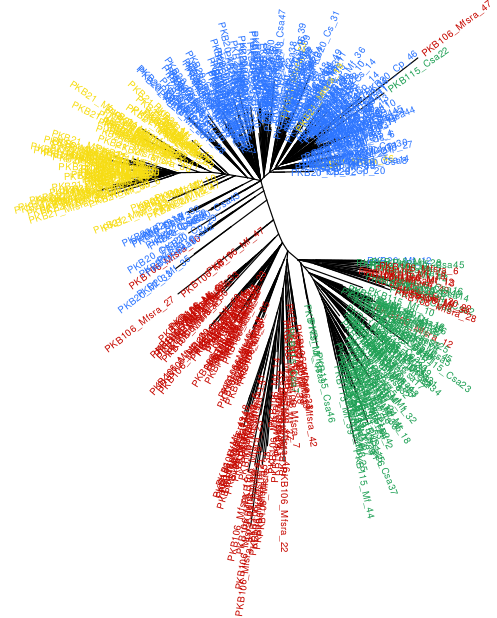
\includegraphics[scale=0.3]{img/pkb_tree.png}				
				\caption{\textbf{Phylogénie des super-familles pK$\beta$:} La super-famille 106 est en rouge, 115 en vert, 20 en bleu et 21 en jaunes.
	\label{fig:pkb_tree}} 
	\end{figure}

	Pour poursuivre l'étude sur les familles communes entre espèces, le regroupement des familles $\alpha$-satellites ayant  le motif pK$\beta$ ou "familles pK$\beta$" attirent l'attention. D'abord sont analysées les familles qui ont le motif à plus de 75\%. Elles représentent au mieux les familles pK$\beta$. Les familles qui expriment moins le motif sont analysées par la suite, pour voir si malgré la faible présence du motif, elles se rassemblent en une ou plusieurs super-familles. Il existe au total 6 SF pK$\beta$.
	
	La première SF pK$\beta$ est constituée de la famille C3 de \textit{C. pogonias}, la famille 3 de \textit{C. sabeus}, et la famille 8 de \textit{M. fascicularis}. La SF 21 est spécifique au macaque, regroupant la famille 1. Toutes ces espèces ont donc une "famille C3" en commun, peut-être sous forme de dimère C2-C3.
	
	Le \textit{M. fascicularis} et \textit{C.sabeus} ont deux SF pK$\beta$ en commun. Les familles constituant ces SF ont un pourcentage du motif relativement faible, pourtant elles sont tout de même rassemblées. 
	
	Le \textit{C.sabeus} et le \textit{M. fascicularis} ont respectivement chacun une SF pK$\beta$ spécifique. La première SF a le motif à 27\% et la deuxième à 50\%.
		
	Un arbre composé de toutes les SF pK$\beta$ est construit pour voir comment elles s'assemblent. Le jeu de données est construit à partir de 50 séquences par famille pK$\beta$ par espèce tirées aléatoirement (Figure \ref{fig:pkb_tree}). Elles se rassemblent exactement comme dans les SF. La méthode de classification retrouve bien les familles pK$\beta$ et elle les classe correctement.

%%%%%%%%%%%%%%%%%%%%%%%%%%%%%%%%%%%%%%%%%%%%%%%%%%%%%%%%%%%%%%%%%%
%%%%%%%%%%%%%%%%%%%%%%%%Discussion%%%%%%%%%%%%%%%%%%%%%%%%%%%%%%%%
%%%%%%%%%%%%%%%%%%%%%%%%%%%%%%%%%%%%%%%%%%%%%%%%%%%%%%%%%%%%%%%%%%
\section{Discussion}

	Nombre de famille par espces est tres variable

	Les tailles moyennes des consensus sont de 173 nucléotides pour \textit{C. pogonias}, 173 pour \textit{C. solatus}, 173 pour le \textit{C. sabaeus} et X pour le \textit{M. fascicularis}\\
	
	Les plus grandes familles C2 de solatus sont regroupées\\


\section{Conclusion}


%%%%%%%%%%%%%%%%%%%%%%%%%%%%%%%%%%%%%%%%%%%%%%%%%%%%%%%%%%%%%%%%%%
%%%%%%%%%%%%%%%%%%%%%%%%Bibliographie%%%%%%%%%%%%%%%%%%%%%%%%%%%%
%%%%%%%%%%%%%%%%%%%%%%%%%%%%%%%%%%%%%%%%%%%%%%%%%%%%%%%%%%%%%%%%%
\newpage
\strut  ~  \mbox{}  \null
\newpage
\bibliographystyle{unsrt} \bibliography{biblio} 

%%%%%%%%%%%%%%%%%%%%%%%%%%%%%%%%%%%%%%%%%%%%%%%%%%%%%%%%%%%%%%%%%%
%%%%%%%%%%%%%%%%%%%%Résumé & Abstract%%%%%%%%%%%%%%%%%%%%%%%%%%%%%
%%%%%%%%%%%%%%%%%%%%%%%%%%%%%%%%%%%%%%%%%%%%%%%%%%%%%%%%%%%%%%%%%%
\newpage 
\thispagestyle{empty}
\section*{Résumé}~\\[0.2cm]
Votre résumé commence ici...
   ...
\section*{Abstract}~\\[0.2cm]
 Abstract begins here...
   ...
\end{document}
